\chapter{Reconhecimento de Lombadas}
\label{cap:deteccao_lombadas}

Nesta seção é apresentado o estudo voltado ao desenvolvimento de um modelo adaptativo para detecção de lombadas na via. Baseado nos experimentos das seções anteriores, este estudo focou no desenvolvimento de modelos baseados em \textit{Deep Learning}. Contudo, nos anteriores foi produzido modelos para classificação multi classe de eventos persistentes, enquanto neste os modelos consistem de uma classificação binária de evento transiente. O processo de desenvolvimento e experimentação é detalhado nas próximas subseções. Na primeira delas, o pré-processamento, foi realizada a seleção de variáveis, padronizado seus dados através de normalização dos sinais, e definido experimentos para avaliar aspectos como ponto de coleta de dados no veículo, tamanho da janela de dados e variações contextuais, onde foi possível analisar a capacidade de generalização do aprendizado dos modelos para contextos desconhecidos e, portanto, avaliar sua adaptabilidade. Na segunda subseção, processamento, foram desenvolvidos cinco modelos de DNN baseados em diferentes técnicas de \textit{Deep Learning}: LSTM, GRU, CNN, CNN-LSTM e ConvLSTM. Por fim, na última subseção são detalhados e comparados os resultados obtidos.

\section{Pré-Processamento}

Com base nos resultados obtidos nos experimentos das seções anteriores, neste estudo utilizamos como características de entrada os dados brutos das variáveis de aceleração em três eixos (X, Y, Z) e em três diferentes pontos de coleta (abaixo e próximo da suspensão, acima e próximo da suspensão e painel de controle), juntamente com os dados de taxa rotação em três eixos e em três diferentes pontos de coleta, além da velocidade do veículo. Inicialmente, todos os dados foram normalizados com \textit{Robust Scaler}, mantendo o sinal de direção do vetor de força. Após a normalização dos dados, para avaliar a influência da propriedade de dependência veicular e verificar a viabilidade de um modelo de classificação para os dados coletados em diferentes pontos do veículo, foram definidos os seguintes \emph{experimentos por colocação}, com base nos pontos de coleta de dados no veículo:

\begin{description}
	
	\item[Experimento por Colocação 1:] Foram utilizados os dados de força de aceleração 3D e taxa de rotação 3D amostrados próximo e abaixo da suspensão, mais a velocidade.
    
    \item[Experimento por Colocação 2:] Foram utilizados os dados de força de aceleração 3D e taxa de rotação 3D amostrados próximo e acima da suspensão, mais a velocidade.
    
    \item[Experimento por Colocação 3:] Foram utilizados os dados de força de aceleração 3D e taxa de rotação 3D amostrados no painel de controle, mais a velocidade.
    
\end{description}

Para avaliar a capacidade de generalização do aprendizado de cada técnica, avaliando sua adaptabilidade para contextos desconhecidos onde há variação nas propriedades de dependência veicular, de condução e ambiental, os dados de treinamento e validação foram divididos da mesma maneira que nos estudos das seções anteriores, separando-os de acordo com o conjunto de dados em três \emph{experimentos por contexto}:

\begin{description}
	
	\item[Experimento por Contexto 1:] O modelo aprende dados de todos os veículos e motoristas para alguns cenários; mas não todos os veículos com todos os motoristas para todos os cenários.
    \begin{itemize}
        \item \textbf{Treinamento (65\%):} PVS 1, PVS 3, PVS 4, PVS 6, PVS 7, PVS 9. 
        \item \textbf{Validação (35\%):} PVS 2, PVS 5, PVS 8.
    \end{itemize}
    
    \item[Experimento por Contexto 2:] O modelo aprende dados de todos os cenários para alguns veículos e alguns motoristas; mas não todos os veículos com todos os motoristas para todos os cenários.
    \begin{itemize}
        \item \textbf{Treinamento (66\%):} PVS 1, PVS 2, PVS 3, PVS 7, PVS 8, PVS 9.
        \item \textbf{Validação (34\%):} PVS 4, PVS 5, PVS 6.
    \end{itemize}
    
    \item[Experimento por Contexto 3:] O modelo aprende dados de alguns veículos com alguns motoristas para alguns cenários; mas não todos os veículos com todos os motoristas para todos os cenários.
    \begin{itemize}
        \item \textbf{Treinamento (66\%):} PVS 1, PVS 2, PVS 4, PVS 6, PVS 8, PVS 9.
        \item \textbf{Validação (34\%):} PVS 3, PVS 5, PVS 7.
    \end{itemize}
    
\end{description}

Neste estudo, para bem avaliar as variações contextuais, além de dados de lombadas em diferentes pavimentos, sendo asfalto e a paralelepípedo, os modelos ainda contam com amostras de vias de terra, as quais são importantes para os modelos minimizarem FP, uma vez que estradas de terra apresentam irregularidades que produzem assinaturas nos sinais semelhantes às produzidas por lombadas, sendo importante que os modelos saibam diferenciá-las. 

Finalmente, para analisar a influência do número de amostras na classificação, foram criados três \emph{experimentos por tamanho de janela de dados}, com janelas de 100, 200, 300, 400, e 500 amostras. A janela de dados utilizada foi deslizante com sobreposição total, e cada amostra correspondeu a um vetor com os valores das características. A aplicação de janela deslizante se mostra importante neste estudo para analisarmos o comportamento do modelo com entrada de dados em diferentes segmentos da lombada, como janelas com amostras do início, meio ou fim do obstáculo. Em resumo, cada experimento realizado neste estudo é um elemento do produto cartesiano entre \emph{experimentos por colocação}, \emph{experimentos por contexto} e \emph{experimentos por tamanho de janela de dados}.

Através da \autoref{table:lombada_metricas} observamos certo desbalanceamento das classes de dados. Sendo assim, se faz necessário analisar o grau desse desbalanceamento, uma vez que classes sub-representadas (\textit{minor data class}) podem não ser adequadamente tratadas pelos modelos, resultando em viés. Para avaliar a necessidade de aplicar técnicas de balanceamento, medimos a proporção de distribuição de cada classe de dados conforme detalhado \autoref{table:distribuicao_classes_lombadas}. A distribuição de classes foi calculada sobre os dados de treinamento, uma vez que são com estes que os modelos aprendem \cite{He2013, Kuhn2013}. A distribuição foi calculada em relação ao tamanho da janela de dados. Sendo assim, o valor detalhado em cada célula corresponde ao limite inferior e superior da distribuição da classe de dados, uma vez que cada tamanho da janela de dados apresenta uma pequena variação deste valor.

\begin{table}[h]
\caption{Distribuição de classes de lombadas}
\label{table:distribuicao_classes_lombadas}
\centering
\scriptsize
\begin{tabular}{lcccc}
\cmidrule(l){2-5}
\multicolumn{1}{c}{\multirow{2}{*}{\textbf{}}} & 
\multicolumn{4}{c}{\textbf{Classe de Dados}} \\ \cmidrule(l){2-5} 
\multicolumn{1}{c}{} & 
\multicolumn{2}{c}{\textbf{CL - Com Lombada}} & 
\multicolumn{2}{c}{\textbf{SL - Sem Lombada}} \\ \midrule
\textbf{Fonte de Dados} & 
\textit{\textbf{Percentual}} & 
\textit{\textbf{Proporção}} & 
\textit{\textbf{Percentual}} & 
\textit{\textbf{Proporção}} \\ \midrule
Exp. por Contexto 1 & 1.61\% - 1.45\% & 1:60.87 - 1:67.76 & 98.39\% - 98.55\% & 1:0.01 - 1:0.02 \\ \midrule
Exp. por Contexto 2 & 1.58\% - 1.36\% & 1:62.03 - 1:72.22 & 98.42\% - 98.64\% & 1:0.01 - 1:0.02 \\ \midrule
Exp. por Contexto 3 & 1.63\% - 1.44\% & 1:60.17 - 1:68.39 & 98.37\% - 98.56\% & 1:0.01 - 1:0.02 \\ \bottomrule
\end{tabular}
\fonte{Desenvolvido pelo autor.}
\end{table}

O desbalanceamento de classes pode ser considerado leve ou severo, onde as proporções de distribuição que variam de 1:4 até 1:100 (presença de 20\% - 1\%) são consideradas desbalanceamento leve e proporções de distribuição que variam de 1:100 ou mais (<1\% de presença) são consideradas desbalanceamentos severos \cite{Krawczyk2016,Brownlee2020}. Analisando a \autoref{table:distribuicao_classes_lombadas}, observamos que ambas as classes de dados apresentam desbalanceamentos leve, mas com alta tendência a desbalanceamentos severo. Para a classe \emph{Com Lombada (CL)}, a proporção varia entre 1:60.17 a 1:72.22, onde para 1 amostra da classe de dados \emph{CL}, há de 60.17 a 72.22 amostras da classe de dados \emph{Sem Lombada (SL)}. Portanto, realizamos \textit{downsampling} nos segmentos de dados sem lombada (\emph{SL}), descartando as janelas de sobreposição. Em suma, os dados onde há lombada contam com janela deslizante com sobreposição total, e onde não há lombada, a janela é fixa sem sobreposição. Com esta abordagem, a distribuição obtida é detalhada na \autoref{table:distribuicao_classes_lombadas_downsampling}, com uma redução da desproporção em aproximadamente 10 vezes.

\begin{table}[h]
\caption{Distribuição de classes de lombadas após \textit{downsampling}}
\label{table:distribuicao_classes_lombadas_downsampling}
\centering
\scriptsize
\begin{tabular}{lcccc}
\cmidrule(l){2-5}
\multicolumn{1}{c}{\multirow{2}{*}{\textbf{}}} & 
\multicolumn{4}{c}{\textbf{Classe de Dados}} \\ \cmidrule(l){2-5} 
\multicolumn{1}{c}{} & 
\multicolumn{2}{c}{\textbf{CL - Com Lombada}} & 
\multicolumn{2}{c}{\textbf{SL - Sem Lombada}} \\ \midrule
\textbf{Fonte de Dados} & 
\textit{\textbf{Percentual}} & 
\textit{\textbf{Proporção}} & 
\textit{\textbf{Percentual}} & 
\textit{\textbf{Proporção}} \\ \midrule
Exp. por Contexto 1 & 88.01\% - 62.12\% & 1:0.14 - 1:0.61 & 37.87\% - 11.99\% & 1:1.64 - 1:7.34 \\ \midrule
Exp. por Contexto 2 & 87.34\% - 61.68\% & 1:0.14 - 1:0.62 & 38.31\% - 12.66\% & 1:1.61 - 1:6.90 \\ \midrule
Exp. por Contexto 3 & 87.86\% - 62.41\% & 1:0.14 - 1:0.60 & 37.59\% - 12.14\% & 1:1.66 - 1:7.28 \\ \bottomrule
\end{tabular}
\fonte{Desenvolvido pelo autor.}
\end{table}

\section{Processamento}

Após o pré-processamento, os dados foram aplicados em cinco modelos de \textit{Deep Learning}, sendo baseados em LSTM, GRU, CNN, CNN-LSTM e ConvLSTM. Todos os modelos desenvolvidos são sequenciais e utilizam o otimizador Adam em conjunto com a função de perda Entropia Cruzada Binária. Todos os modelos tiveram seus hiperparâmetros ajustados (\textit{hyperparameter tuning}) utilizando o algoritmo \textit{HyperBand} implementado na biblioteca Keras Tuner, onde foram testados diferentes tipos de camadas, número de camadas e neurônios, funções de ativação e várias outras características para encontrar o conjunto ideal de hiper-parâmetros para cada DNN. 

O melhor modelo baseado em LSTM obtido através do ajuste de hiper-parâmetros é detalhado na \autoref{fig:best_lstm_tipo_lombadas}. O modelo DNN é composto de um bloco de camada de entrada, três blocos de camadas de recorrência e regularização e dois blocos de camada totalmente conectados para produção de saída. O bloco de entrada possui uma camada que recebe um tensor \emph{janelas x sequências x características}, onde \emph{janelas} são os agrupamentos de todas as janelas de dados, \emph{sequências} são as sequências de dados para cada janela, e \emph{características} são os valores das variáveis de entrada. Cada bloco de recorrência e regularização é composto por uma camada LSTM bidirecional de 128 unidades, seguida por uma camada de \textit{Batch Normalization} e uma camada de \textit{Dropout} em 25\%. Após o processamento nas camadas recorrentes, os parâmetros são passados para os blocos totalmente conectados, onde existem duas camadas \textit{Dense}, a primeira com 128 neurônios e ativação \textit{Relu}, e a segunda com 1 neurônio e ativação \textit{Sigmoid}. A saída produzida é uma resposta binária à presença ou ausência de lombadas na janela de dados. A saída esperada são os rótulos mais presentes na janela de dados.

\begin{figure}[h!]
  \centering
  \caption{Modelo LSTM para detecção de lombadas}
  \label{fig:best_lstm_tipo_lombadas}
  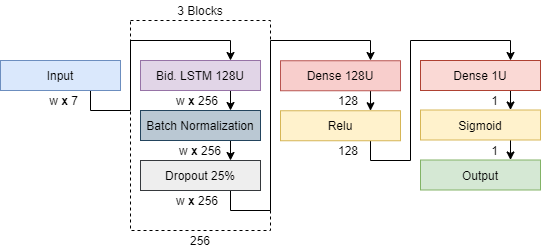
\includegraphics[width=0.75\textwidth]{figuras/fig_40.png}
 \fonte{Desenvolvido pelo autor.}
\end{figure}

O melhor modelo baseado em GRU obtido neste estudo está detalhado na \autoref{fig:best_gru_tipo_lombadas}. O modelo de DNN é composto de um bloco de camada de entrada, dois blocos de camadas de recorrência e regularização e dois blocos de camadas totalmente conectadas para produção de saída. O bloco de entrada possui uma camada que recebe um tensor \emph{janelas x sequências x características}, semelhante ao baseado em LSTM. Cada bloco de recorrência e regularização é composto por uma camada GRU bidirecional de 192 unidades, seguida por uma camada de \textit{Batch Normalization} e uma camada de \textit{Dropout} em 20\%. Após o processamento nas camadas recorrentes, os parâmetros passam para um bloco totalmente conectado, onde existem duas camadas \textit{Dense}, a primeira com 192 neurônios e ativação \textit{Relu}, e a segunda com 1 neurônio e ativação \textit{Sigmoid}, produzindo a resposta binária.

\begin{figure}[h!]
  \centering
  \caption{Modelo GRU para detecção de lombadas}
  \label{fig:best_gru_tipo_lombadas}
  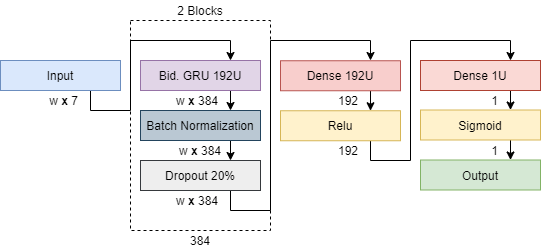
\includegraphics[width=0.75\textwidth]{figuras/fig_41.png}
 \fonte{Desenvolvido pelo autor.}
\end{figure}

O melhor modelo baseado em CNN obtido é detalhado na \autoref{fig:best_cnn_tipo_lombadas}. O modelo de DNN é composto de um bloco de entrada, dois blocos de convolução e regularização e dois blocos de camadas totalmente conectadas para produção de saída. O bloco de entrada possui uma camada que recebe um tensor \emph{janelas x sequências x características}, semelhante aos modelos baseados em LSTM e GRU. O primeiro bloco de convolução e regularização é composto por uma camada Conv 1D com 224 filtros com \textit{kernel} de tamanho 5 para extração de características e ativação \textit{Relu}, seguida de regularização através de uma camada de \textit{Batch Normalization} e uma camada de \textit{Spatial Dropout 1D} em 50\%. O último bloco de convolução e regularização tem uma camada Conv 1D com as mesmas configurações da anterior, uma camada \textit{Global Max Pooling 1D} para extrair recursos mais robustos por meio dos valores máximos em cada região, e camadas de regularização por \textit{Batch Normalization} e \textit{Dropout} em 50\%. Finalmente, os blocos totalmente conectados consistem em duas camadas \textit{Dense}, uma com 160 neurônios e ativação \textit{Relu} e outra com 1 neurônio e ativação \textit{Sigmoid}, produzindo a saída binária.

\begin{figure}[h!]
  \centering
  \caption{Modelo CNN para detecção de lombadas}
  \label{fig:best_cnn_tipo_lombadas}
  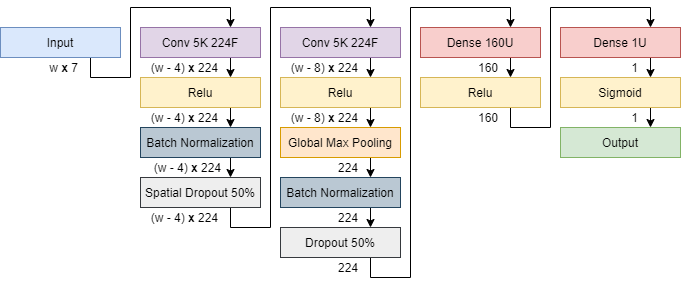
\includegraphics[width=0.9\textwidth]{figuras/fig_42.png}
 \fonte{Desenvolvido pelo autor.}
\end{figure}

\begin{figure}[h!]
  \centering
  \caption{Modelo CNN-LSTM para detecção de lombadas}
  \label{fig:best_cnn_lstm_tipo_lombadas}
  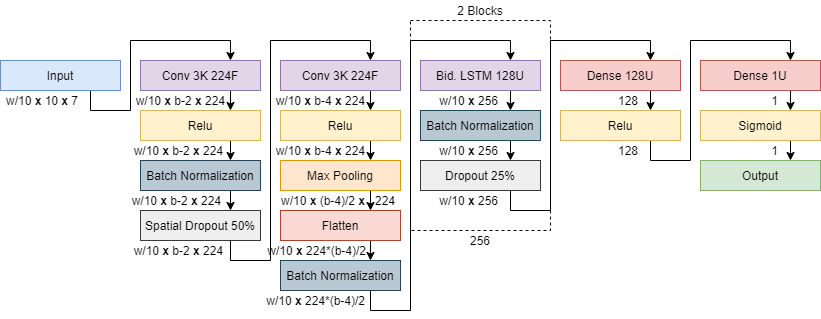
\includegraphics[width=1\textwidth]{figuras/fig_43.png}
 \fonte{Desenvolvido pelo autor.}
\end{figure}

O melhor modelo híbrido baseado em CNN-LSTM obtido é detalhado na \autoref{fig:best_cnn_lstm_tipo_lombadas}. O modelo de DNN baseado em CNN-LSTM desenvolvido é composto de um bloco de entrada, dois blocos de convolução e regularização, dois blocos recorrentes e de regularização e dois blocos de camada totalmente conectadas para produção de saída. O bloco de entrada tem uma camada que recebe um tensor \emph{janelas x sequências x subsequências x características}, onde \emph{janelas} são os agrupamentos de todas as janelas de dados, \emph{sequências} são as sequências de dados para cada janela, \emph{subsequências} são as subpartes da sequência de dados original, e \emph{características} os valores das variáveis de entrada. O primeiro bloco de convolução e regularização é composto por uma camada Conv 1D com 224 filtros com  \textit{kernel} de tamanho 3 para extração de características e ativação \textit{Relu}, seguida de regularização através de uma camada de \textit{Batch Normalization} e uma camada de \textit{Spatial Dropout 1D} em 50\%. O último bloco de convolução e regularização tem uma camada Conv 1D com as mesmas configurações da anterior, uma camada \textit{Max Pooling 1D} para extrair recursos mais robustos por meio dos valores máximos em cada região, uma camada \textit{Flatten} para reagrupar os recursos extraídos na sequência temporal original, e regularização por camada de \textit{Batch Normalization}. Em seguida, cada bloco de recorrência e regularização é composto por uma camada LSTM bidirecional de 128 unidades, seguida por uma camada de \textit{Batch Normalization} e uma camada de \textit{Dropout} em 25\%. Finalmente, os parâmetros resultantes passam para duas camadas \textit{Dense}, a primeira com 128 neurônios e ativação de \textit{Relu}, e a segunda com 1 neurônio e ativação de \textit{Sigmoid}, produzindo a saída binária. 

O melhor modelo baseado em ConvLSTM obtido é detalhado na Figura \autoref{fig:best_conv_lstm_tipo_lombadas}. O modelo DNN é composto de um bloco de entrada, dois blocos convolucionais recorrentes e de regularização, e dois blocos de camadas totalmente conectadas para produção de saída. O bloco de entrada possui uma camada que recebe um tensor \emph{janelas x sequências x subsequências x características}, semelhante ao modelo CNN-LSTM. Os dois blocos convolucionais recorrentes e de regularização são compostos por uma camada \textit{ConvLSTM 1D} com 224 filtros \textit{kernel} de tamanho 3 e ativação \textit{Relu}, seguido por regularização através de uma camada \textit{Dropout} em 30\%. Finalmente, os parâmetros resultantes são achatados (\textit{flattened)} e passados para duas camadas \textit{Dense}, a primeira com 224 neurônios e ativação \textit{Relu}, e a segunda com 1 neurônio e ativação \textit{Sigmoid}, produzindo a saída binária.

\begin{figure}[h!]
  \centering
  \caption{Modelo ConvLSTM para detecção de lombadas}
  \label{fig:best_conv_lstm_tipo_lombadas}
  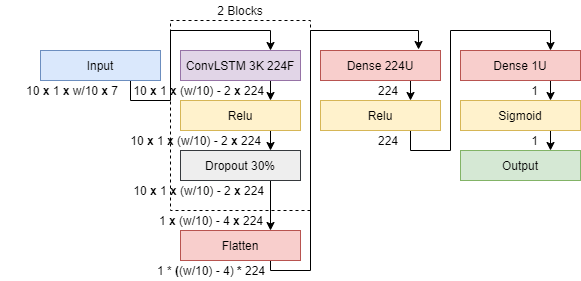
\includegraphics[width=0.8\textwidth]{figuras/fig_44.png}
 \fonte{Desenvolvido pelo autor.}
\end{figure}

\section{Análise de Resultados}

Neste estudo todos os modelos de detecção de lombadas foram desenvolvidos na linguagem Python 3, utilizando da biblioteca Keras 2, a qual é uma API de alto nível do TensorFlow. Os hiperparâmetros dos modelos foram afinados através da biblioteca Keras Tuner. Todos os experimentos foram executados em máquinas do Google \textit{Collaboratory}, de mesma configuração dos estudos das seções anteriores. Cada experimento é um elemento do produto Cartesiano entre \emph{experimentos por colocação}, \emph{experimentos por contexto} e \emph{experimentos por tamanho da janela de dados}, sendo executado três vezes e recuperando-se o melhor das três execuções. Consideramos a melhor execução aquela com maior valor de acurácia na fase de validação, uma vez que o treinamento dos modelos foi configurado para maximizar a métrica de acurácia.

Os resultados obtidos com a execução de todos os experimentos são apresentados nas Tabelas \ref{table:lstm_accuracy_result_lombadas}-\ref{table:conv_lstm_accuracy_result_lombadas}. Em cada tabela são detalhados os resultados para determinado modelo de DNN, para cada colocação, contexto e janela de dados. Também são apresentadas métricas de média aritmética para cada tipo de experimento, sendo Acurácia Média dos Experimentos por Contexto (AMEC) e Acurácia Média dos Experimentos por Contexto e Colocação (AMECC), onde são destacados os menores e maiores valores de acurácia obtidos na fase de validação.

\begin{table}[H]
\scriptsize
\centering
\caption{Valores de acurácia em validação obtidos pelo modelo LSTM} 
\label{table:lstm_accuracy_result_lombadas}
\begin{tabular}{ccccccc}
\toprule
\multicolumn{2}{c}{\textbf{Tipo de Experimento}} & \multicolumn{5}{c}{\textit{\textbf{Tamanho da Janela de Dados}}} \\ \midrule
\textit{\textbf{Colocação}} & \textit{\textbf{Contexto}} & \textit{100} & \textit{200} & \textit{300} & \textit{400} & \textit{500} \\ \midrule
\multirow{4}{*}{\begin{tabular}[c]{@{}c@{}} \\ Próximo e Abaixo \\ da Suspensão\end{tabular}} 
& 1 & 95.03\% & 96.53\% & 98.59\% & 99.18\% & 99.21\% \\ \cmidrule(l){2-7} 
& 2 & 90.70\% & 94.33\% & 97.08\% & 97.12\% & 97.81\% \\ \cmidrule(l){2-7} 
& 3 & 95.05\% & 97.54\% & 98.66\% & 99.12\% & 98.52\% \\ \cmidrule(l){2-7} 
& AMEC & \cellcolor[HTML]{FFCCC9}93.59\% & 96.13\% & 98.11\% & 98.47\% & \cellcolor[HTML]{34FF34}98.52\% \\ \midrule
\multirow{4}{*}{\begin{tabular}[c]{@{}c@{}} \\ Próximo e Acima \\ da Suspensão\end{tabular}} 
& 1 & 92.77\% & 93.68\% & 97.83\% & 98.97\% & 98.46\% \\ \cmidrule{2-7} 
& 2 & 92.90\% & 94.98\% & 97.21\% & 97.76\% & 97.66\% \\ \cmidrule{2-7} 
& 3 & 95.00\% & 96.64\% & 98.60\% & 99.25\% & 99.30\% \\ \cmidrule{2-7} 
& AMEC & \cellcolor[HTML]{FFCCC9}93.56\% & 95.10\% & 97.88\% & \cellcolor[HTML]{34FF34}98.66\% & 98.47\%   \\ \midrule
\multirow{4}{*}{\begin{tabular}[c]{@{}c@{}} \\ Painel de Controle \end{tabular}} 
& 1 & 93.99\% & 94.55\% & 99.22\% & 98.77\% & 98.18\% \\ \cmidrule{2-7} 
& 2 & 92.10\% & 95.70\% & 97.37\% & 97.38\% & 98.48\% \\ \cmidrule{2-7} 
& 3 & 95.19\% & 97.36\% & 99.24\% & 99.33\% & 98.62\% \\ \cmidrule{2-7} 
& AMEC & \cellcolor[HTML]{FFCCC9}93.76\% & 95.87\% & \cellcolor[HTML]{34FF34}98.61\% & 98.49\% & 98.43\%  \\ \midrule
& AMECC & \cellcolor[HTML]{FFCCC9}93.64\% & 95.70\% & 98.20\% & \cellcolor[HTML]{34FF34}98.54\% & 98.47\% \\ \cmidrule(l){2-7} 
\end{tabular}
\fonte{Desenvolvido pelo autor.}
\end{table}

\begin{table}[H]
\scriptsize
\centering
\caption{Valores de acurácia em validação obtidos pelo modelo GRU} 
\label{table:gru_accuracy_result_lombadas}
\begin{tabular}{ccccccc}
\toprule
\multicolumn{2}{c}{\textbf{Tipo de Experimento}} & \multicolumn{5}{c}{\textit{\textbf{Tamanho da Janela de Dados}}} \\ \midrule
\textit{\textbf{Colocação}} & \textit{\textbf{Contexto}} & \textit{100} & \textit{200} & \textit{300} & \textit{400} & \textit{500} \\ \midrule
\multirow{4}{*}{\begin{tabular}[c]{@{}c@{}} \\ Próximo e Abaixo \\ da Suspensão\end{tabular}} 
 & 1 & 94.23\% & 96.42\% & 97.84\% & 98.60\% & 95.78\% \\ \cmidrule{2-7} 
 & 2 & 92.76\% & 94.20\% & 96.83\% & 96.54\% & 97.25\% \\ \cmidrule{2-7} 
 & 3 & 94.46\% & 97.54\% & 98.55\% & 98.88\% & 96.17\% \\ \cmidrule{2-7} 
 & AMEC & \cellcolor[HTML]{FFCCC9}93.82\% & 96.05\% & 97.74\% & \cellcolor[HTML]{34FF34}98.01\% & 96.40\% \\ \midrule
\multirow{4}{*}{\begin{tabular}[c]{@{}c@{}} \\ Próximo e Acima \\ da Suspensão\end{tabular}} 
 & 1 & 93.57\% & 93.61\% & 98.23\% & 94.44\% & 95.45\% \\ \cmidrule{2-7} 
 & 2 & 90.93\% & 94.17\% & 97.17\% & 97.39\% & 96.45\% \\ \cmidrule{2-7} 
 & 3 & 93.90\% & 96.82\% & 98.53\% & 98.00\% & 98.62\% \\ \cmidrule{2-7} 
 & AMEC & \cellcolor[HTML]{FFCCC9}92.80\% & 94.87\% & \cellcolor[HTML]{34FF34}97.98\% & 96.61\% & 96.84\% \\ \midrule
\multirow{4}{*}{\begin{tabular}[c]{@{}c@{}} \\ Painel de Controle \end{tabular}} 
 & 1 & 94.41\% & 96.78\% & 97.94\% & 96.88\% & 95.92\% \\ \cmidrule{2-7} 
 & 2 & 92.05\% & 96.37\% & 96.91\% & 98.05\% & 93.01\% \\ \cmidrule{2-7} 
 & 3 & 94.64\% & 96.93\% & 98.54\% & 99.18\% & 97.38\% \\ \cmidrule{2-7} 
 & AMEC & \cellcolor[HTML]{FFCCC9}93.70\% & 96.69\% & 97.80\% & \cellcolor[HTML]{34FF34}98.04\% & 95.44\% \\ \midrule
& AMECC  & \cellcolor[HTML]{FFCCC9}93.44\% & 95.87\% & \cellcolor[HTML]{34FF34}97.84\% & 97.55\% & 96.23\% \\ \cmidrule(l){2-7} 
\end{tabular}
\fonte{Desenvolvido pelo autor.}
\end{table}

\begin{table}[H]
\scriptsize
\centering
\caption{Valores de acurácia em validação obtidos pelo modelo CNN} 
\label{table:cnn_accuracy_result_lombadas}
\begin{tabular}{ccccccc}
\toprule
\multicolumn{2}{c}{\textbf{Tipo de Experimento}} & \multicolumn{5}{c}{\textit{\textbf{Tamanho da Janela de Dados}}} \\ \midrule
\textit{\textbf{Colocação}} & \textit{\textbf{Contexto}} & \textit{100} & \textit{200} & \textit{300} & \textit{400} & \textit{500} \\ \midrule
\multirow{4}{*}{\begin{tabular}[c]{@{}c@{}} \\ Próximo e Abaixo \\ da Suspensão\end{tabular}} 
 & 1 & 94.20\% & 95.12\% & 97.38\% & 97.45\% & 99.8\% \\ \cmidrule{2-7} 
 & 2 & 91.02\% & 90.57\% & 93.32\% & 95.33\% & 95.73\% \\ \cmidrule{2-7} 
 & 3 & 95.55\% & 96.07\% & 97.62\% & 98.32\% & 99.36\% \\ \cmidrule{2-7} 
 & AMEC & \cellcolor[HTML]{FFCCC9}93.59\% & 93.92\% & 96.11\% & 97.03\% & \cellcolor[HTML]{34FF34}98.30\% \\ \midrule
\multirow{4}{*}{\begin{tabular}[c]{@{}c@{}} \\ Próximo e Acima \\ da Suspensão\end{tabular}} 
 & 1 & 95.1\% & 96.08\% & 97.18\% & 97.55\% & 98.85\% \\ \cmidrule{2-7} 
 & 2 & 93.77\% & 94.40\% & 96.96\% & 97.66\% & 97.11\% \\ \cmidrule{2-7} 
 & 3 & 95.11\% & 95.94\% & 98.67\% & 99.40\% & 97.84\% \\ \cmidrule{2-7} 
 & AMEC & \cellcolor[HTML]{FFCCC9}94.66\% & 95.48\% & 97.60\% & \cellcolor[HTML]{34FF34}98.20\% & 97.93\% \\ \midrule
\multirow{4}{*}{\begin{tabular}[c]{@{}c@{}} \\ Painel de Controle \end{tabular}} 
 & 1 & 95.41\% & 95.69\% & 97.61\% & 97.84\% & 99.78\% \\ \cmidrule{2-7} 
 & 2 & 94.43\% & 93.59\% & 96.24\% & 97.19\% & 97.41\% \\ \cmidrule{2-7} 
 & 3 & 95.57\% & 95.11\% & 97.51\% & 98.52\% & 98.96\% \\ \cmidrule{2-7} 
 & AMEC & 95.14\% & \cellcolor[HTML]{FFCCC9}94.80\% & 97.12\% & 97.85\% & \cellcolor[HTML]{34FF34}98.72\% \\ \midrule
 & AMECC & \cellcolor[HTML]{FFCCC9}94.46\% & 94.73\% & 96.94\% & 97.69\% & \cellcolor[HTML]{34FF34}98.32\% \\ \cmidrule(l){2-7} 
\end{tabular}
\fonte{Desenvolvido pelo autor.}
\end{table}

\begin{table}[H]
\scriptsize
\centering
\caption{Valores de acurácia em validação obtidos pelo modelo CNN-LSTM} 
\label{table:cnn_lstm_accuracy_result_lombadas}
\begin{tabular}{ccccccc}
\toprule
\multicolumn{2}{c}{\textbf{Tipo de Experimento}} & \multicolumn{5}{c}{\textit{\textbf{Tamanho da Janela de Dados}}} \\ \midrule
\textit{\textbf{Colocação}} & \textit{\textbf{Contexto}} & \textit{100} & \textit{200} & \textit{300} & \textit{400} & \textit{500} \\ \midrule
\multirow{4}{*}{\begin{tabular}[c]{@{}c@{}} \\ Próximo e Abaixo \\ da Suspensão\end{tabular}} 
 & 1 & 94.49\% & 96.76\% & 98.95\% & 99.08\% & 98.20\% \\ \cmidrule{2-7} 
 & 2 & 94.30\% & 94.63\% & 96.83\% & 97.72\% & 96.79\% \\ \cmidrule{2-7} 
 & 3 & 95.13\% & 97.75\% & 98.89\% & 98.92\% & 98.93\% \\ \cmidrule{2-7} 
 & AMEC & \cellcolor[HTML]{FFCCC9}94.64\% & 96.38\% & 98.22\% & \cellcolor[HTML]{34FF34}98.57\% & 97.97\% \\ \midrule
\multirow{4}{*}{\begin{tabular}[c]{@{}c@{}} \\ Próximo e Acima \\ da Suspensão\end{tabular}} 
 & 1 & 94.14\% & 96.63\% & 98.75\% & 99.25\% & 99.79\% \\ \cmidrule{2-7} 
 & 2 & 92.78\% & 94.99\% & 97.33\% & 97.39\% & 97.67\% \\ \cmidrule{2-7} 
 & 3 & 94.92\% & 96.77\% & 99.21\% & 99.11\% & 99.38\% \\ \cmidrule{2-7} 
 & AMEC & \cellcolor[HTML]{FFCCC9}93.95\% & 96.13\% & 98.43\% & 98.59\% & \cellcolor[HTML]{34FF34}98.94\% \\ \midrule
\multirow{4}{*}{\begin{tabular}[c]{@{}c@{}} \\ Painel de Controle \end{tabular}} 
 & 1 & 94.18\% & 96.46\% & 99.1\% & 99.22\% & 99.73\% \\ \cmidrule{2-7} 
 & 2 & 92.74\% & 96.2\% & 97.37\% & 97.44\% & 97.46\% \\ \cmidrule{2-7} 
 & 3 & 94.86\% & 96.89\% & 99.13\% & 98.76\% & 99.41\% \\ \cmidrule{2-7} 
 & AMEC & \cellcolor[HTML]{FFCCC9}93.93\% & 96.52\% & 98.53\% & 98.48\% & \cellcolor[HTML]{34FF34}98.87\% \\ \midrule
 & AMECC & \cellcolor[HTML]{FFCCC9}94.17\% & 96.34\% & 98.39\% & 98.55\% & \cellcolor[HTML]{34FF34}98.59\% \\ \cmidrule(l){2-7} 
\end{tabular}
\fonte{Desenvolvido pelo autor.}
\end{table}

\begin{table}[H]
\scriptsize
\centering
\caption{Valores de acurácia em validação obtidos pelo modelo ConvLSTM} 
\label{table:conv_lstm_accuracy_result_lombadas}
\begin{tabular}{ccccccc}
\toprule
\multicolumn{2}{c}{\textbf{Tipo de Experimento}} & \multicolumn{5}{c}{\textit{\textbf{Tamanho da Janela de Dados}}} \\ \midrule
\textit{\textbf{Colocação}} & \textit{\textbf{Contexto}} & \textit{100} & \textit{200} & \textit{300} & \textit{400} & \textit{500} \\ \midrule
\multirow{4}{*}{\begin{tabular}[c]{@{}c@{}} \\ Próximo e Abaixo \\ da Suspensão\end{tabular}} 
 & 1 & 93.77\% & 96.21\% & 97.91\% & 98.43\% & 98.30\% \\ \cmidrule{2-7} 
 & 2 & 91.57\% & 94.92\% & 97.19\% & 96.22\% & 95.93\% \\ \cmidrule{2-7} 
 & 3 & 94.82\% & 96.73\% & 98.57\% & 98.74\% & 97.12\% \\ \cmidrule{2-7} 
 & AMEC & \cellcolor[HTML]{FFCCC9}93.39\% & 95.95\% & \cellcolor[HTML]{34FF34}97.89\% & 97.79\% & 97.12\% \\ \midrule
\multirow{4}{*}{\begin{tabular}[c]{@{}c@{}} \\ Próximo e Acima \\ da Suspensão\end{tabular}} 
 & 1 & 92.92\% & 96.12\% & 97.86\% & 98.21\% & 98.95\% \\ \cmidrule{2-7} 
 & 2 & 92.72\% & 96.60\% & 97.65\% & 96.93\% & 97.52\% \\ \cmidrule{2-7} 
 & 3 & 94.24\% & 96.39\% & 98.48\% & 99.30\% & 99.17\% \\ \cmidrule{2-7} 
 & AMEC & \cellcolor[HTML]{FFCCC9}93.29\% & 96.37\% & 98.00\% & 98.15\% & \cellcolor[HTML]{34FF34}98.55\% \\ \midrule
\multirow{4}{*}{\begin{tabular}[c]{@{}c@{}} \\ Painel de Controle \end{tabular}} 
 & 1 & 94.95\% & 96.68\% & 98.41\% & 99.28\% & 98.79\% \\ \cmidrule{2-7} 
 & 2 & 93.25\% & 95.90\% & 97.31\% & 98.92\% & 98.36\% \\ \cmidrule{2-7} 
 & 3 & 95.04\% & 97.36\% & 98.77\% & 99.35\% & 99.66\% \\ \cmidrule{2-7} 
 & AMEC & \cellcolor[HTML]{FFCCC9}94.41\% & 96.65\% & 98.16\% & \cellcolor[HTML]{34FF34}99.18\% & 98.94\% \\ \midrule
 & AMECC & \cellcolor[HTML]{FFCCC9}93.70\% & 96.32\% & 98.02\% & \cellcolor[HTML]{34FF34}98.37\% & 98.20\% \\ \cmidrule(l){2-7} 
\end{tabular}
\fonte{Desenvolvido pelo autor.}
\end{table}

Em nossa análise, para avaliar a habilidade dos modelos generalizarem seu aprendizado para contextos desconhecidos, como diferentes veículos, motoristas ou ambientes, consideramos que o modelo deve obter bom desempenho nos três \emph{experimentos por contexto}. Sendo assim, nossa análise é pautada inicialmente na média de acurácia destes experimentos, representada pela métrica AMEC. Através dos valores AMEC detalhados nas Tabelas \ref{table:lstm_accuracy_result_lombadas}-\ref{table:conv_lstm_accuracy_result_lombadas}, observamos que todos os modelos de DNN desenvolvidos obtiveram bons resultados independentes do contexto, com o valor de média de acurácia variando entre 92.80\% e 99.18\% conforme modelo e ponto de coleta de dados.

Analisando o impacto do tamanho das janelas de dados, observamos que as janelas de 100 e 200 amostras obtiveram todos os piores resultados para todos os experimentos e modelos, denotando ser uma quantidade de amostras insuficientes para reconhecer lombadas com uma boa confiabilidade. Nestas duas janelas estão as maiores variações dos valores de acurácia, onde a janela de dados de 100 amostras obteve acurácia média de 93.70\%, e a de 200 amostras obteve 95.87\%. Por outro lado, as janelas de 300, 400 e 500 amostras obtiveram os melhores resultados, com uma estabilização dos valores de acurácia, apresentando uma variação muito pequena. Na média entre todos os experimentos e modelos, a janela de 300 amostras obteve acurácia de 98.02\%, a de 400 obteve 98.37\%, e a de 500 obteve 98.32\%. Neste estudo, uma lombada inteira possuí entre 223 a 419 amostras. Logo, podemos concluir que os modelos necessitam de que a janela de dados contenha a lombada por inteiro o muito próximo disso para obter melhores resultados.

Em relação aos pontos de coleta de dados, todos obtiveram bons resultados, com pequena variação de uma colocação para outra. Os valores de média acurácia AMEC entre os modelos para a colocação próximo e abaixo da suspensão variaram de 93.39\% até 98.57\%; para próximo e acima da suspensão de 92.80\% até 98.94\%; e no painel de controle de 93.70\% até 99.18\%. A escolha do melhor modelo neste ponto pode levar em consideração a aplicação final, onde o modelo baseado em CNN-LSTM se mostra melhor para quando os sensores são empregados próximo e abaixo da suspensão ou próximo e acima da suspensão, enquanto que o modelo baseado em ConvLSTM se mostra melhor para aplicação no painel de controle. Contudo, neste estudo consideramos que o melhor modelo deve possibilitar sua operação independentemente do local de colocação dos sensores no veículo. Portanto, deve ser aquele com melhor desempenho entre os diferentes pontos de coleta, representado pela média de acurácia entre os \emph{experimentos por colocação}. Sendo assim, esta métrica é detalhada nas tabelas por AMECC, onde para determinar a melhor configuração de janela para cada modelo é considerado a média de acurácia entre todos os \emph{experimentos por colocação} e \emph{experimentos por contexto}.

Através da métrica supracitada, observamos que o melhor modelo é o baseado em CNN-LSTM em janela de 500 amostras, resultando em média de acurácia de 98.59\%. O segundo melhor é o baseado em LSTM com 400 amostras resultando em 98.54\%. O terceiro o baseado em ConvLSTM de 400 amostras com 98.37\%. Em quarto o baseado em CNN de 500 amostras com 98.32\%. Por último, o modelo baseado em GRU de 300 amostras resultando em 97.84\%. A melhor configuração de cada modelo é detalhada na Tabela \ref{table:best_models_metrics_lombadas} com as demais métricas de avaliação. Todos os valores das métricas apresentadas nesta tabela correspondem a média entre os \emph{experimentos por colocação} e \emph{experimentos por contexto}.

\begin{table}[H]
\scriptsize
\centering
\caption{Métricas de avaliação para a melhor configuração de cada modelo DNN} 
\label{table:best_models_metrics_lombadas}
\begin{tabular}{ccccccc}
\toprule
\multirow{2}{*}{\textbf{\begin{tabular}[c]{@{}c@{}}Métrica de \\ Avaliação\end{tabular}}} & \textbf{Modelo} & LSTM & GRU & CNN & CNN-LSTM & ConvLSTM \\ \cmidrule(l){2-7} 
 & \textbf{Janela} & 400 & 300 & 500 & 500 & 400 \\ \midrule
\multirow{2}{*}{Acurácia} 
 & Treinamento & 99.21\% & 99.71\% & 99.11\% & 99.53\% & 99.56\% \\ \cmidrule{2-7} 
 & Validação & 98.54\% & 97.84\% & 98.32\% & \cellcolor[HTML]{34FF34}98.59\% & 98.37\%  \\ \midrule
\multirow{3}{*}{\begin{tabular}[c]{@{}c@{}} \\ Precisão\end{tabular}} 
 & CL & 99.25\% & 99.64\% & \cellcolor[HTML]{34FF34}99.67\% & 99.64\% & 99.22\% \\ \cmidrule{2-7} 
 & SL & \cellcolor[HTML]{34FF34}94.40\% & 90.40\% & 90.57\% & 92.34\% & 93.49\% \\ \cmidrule{2-7} 
 & Média & \cellcolor[HTML]{34FF34}96.83\% & 95.02\% & 95.12\% & 95.99\% & 96.36\% \\ \midrule
\multirow{3}{*}{\begin{tabular}[c]{@{}c@{}} \\ Recall\end{tabular}} 
 & CL & \cellcolor[HTML]{34FF34}99.06\% & 97.73\% & 98.40\% & 98.75\% & 98.89\% \\ \cmidrule{2-7} 
 & SL & 95.32\% & \cellcolor[HTML]{34FF34}98.36\% & 97.83\% & 97.59\% & 95.13\% \\ \cmidrule{2-7} 
 & Média & 97.19\% & 98.05\% & 98.12\% & \cellcolor[HTML]{34FF34}98.17\% & 97.01\% \\ \midrule
\multirow{3}{*}{\begin{tabular}[c]{@{}c@{}} \\ F1-Score\end{tabular}} 
 & CL & 99.15\% & 98.67\% & 99.02\% & \cellcolor[HTML]{34FF34}99.19\% & 99.05\% \\ \cmidrule{2-7} 
 & SL & \cellcolor[HTML]{34FF34}94.77\% & 94.18\% & 93.83\% & 94.74\% & 94.18\% \\ \cmidrule{2-7} 
 & Média & 96.96\% & 96.43\% & 96.43\% & \cellcolor[HTML]{34FF34}96.97\% & 96.62\%  \\ \bottomrule
\end{tabular}
\fonte{Desenvolvido pelo autor.}
\end{table}

Na \autoref{table:best_models_metrics_lombadas} são apresentadas as métricas de acurácia, precisão, \textit{recall} e \textit{f1-score} para cada melhor configuração dos modelos. Embora a acurácia seja amplamente utilizada, em conjuntos de dados com desbalanceamento ela pode esconder viés, especialmente quando a classe minoritária não é bem tratada pelo modelo \cite{He2013}. Para isto são utilizadas as métricas de avaliação precisão, \textit{recall} e \textit{f1-score}, analisando a performance do modelo em cada classe de dados. Na tabela, para cada métrica são apresentadas os valores para as duas classes de dados deste estudo: \emph{Com Lombada} (CL) e \emph{Sem Lombada} (SL). Como podemos observar, todas as classes de dados foram corretamente tratadas por todos os modelos sem haver viés, de forma que a técnica de \textit{downsampling} empregada foi efetiva. Todas as métricas obtiveram valores acima de 90\%. Neste estudo, consideramos que o melhor modelo deve ser aquele que maximize tanto os VP quanto os VN, e minimize os FN e FP. Desta forma, o modelo deve ter a melhor performance tanto na detecção correta de lombadas quanto a detecção correta de não lombadas. Sendo assim, a métrica de \textit{f1-score} associa estes dois fatores, e na média para as duas classes de dados o modelo baseado em CNN-LSTM com janela de 500 amostras foi o que obteve melhor resultado. Portanto, consideramos o modelo baseado em CNN-LSTM o melhor modelo para detecção de lombadas, com valor de média entre \emph{experimentos por colocação} e \emph{experimentos por contexto} de 98.59\% para acurácia, 95.99\% para precisão, 98.17\% para \textit{recall} e 96.97\% para \textit{f1-score}. Na \autoref{fig:cnn_lstm_confusion_matrix_lombadas} é ilustrado a matriz confusão para o modelo baseado em CNN-LSTM em cada ponto de coleta de dados.

\begin{figure}[H]
  \centering
  \caption{Matriz de confusão para o modelo CNN-LSTM em cada ponto de coleta de dados}
  \label{fig:cnn_lstm_confusion_matrix_lombadas}
  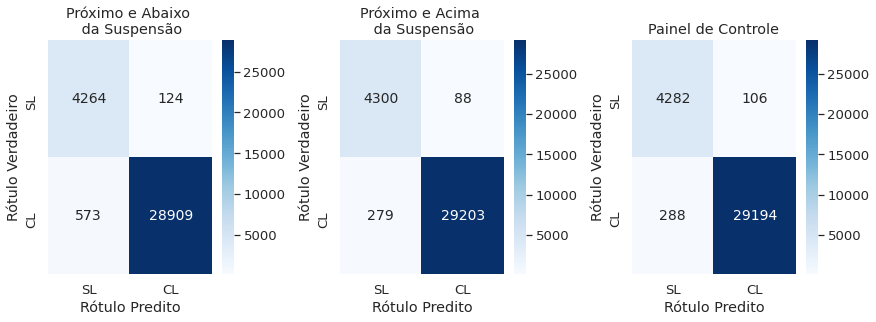
\includegraphics[width=1\textwidth]{figuras/fig_45.png}
  \fonte{Desenvolvido pelo autor.}
\end{figure}

